%!TEX root = main.tex


In this chapter the architecture of the system will be described. The 4+1 model will be used. We will be describing  the logical view, the physical view, the process view and the data view. 
The logical view shows the functional decomposition of the architecture into components.
the process view shows behavioral aspects of the system, the data flow view defines the data, the relation
between data entities, how the data flows through the system and the measures to ensure reliability and
performance. The physical view shows the physical entities and storage units as well as the deployment
scenario.

\section{Logical View}
This view shows the connections between structural elements, key abstractions and mechanisms that are used within SFM. At first, an overview of the components is provided. The main components of the system will be displayed in terms of layers. Next, the main components are decomposed a in term of responsibilities and interfaces.

\subsection{Primary presentation}
In order to design the software architecture of \ac{ET}, the layers pattern is used. This pattern is best suitable for the system since it gives the opportunity to abstract layers from one another, which increases the availability of the system by modularizing the components. The modularization of the components increases also the scalability and the performance of the system. 
The system has been structured according to the three-layers approach. The three main components: Mobile app, Beacon Interface and the Local Storage, and Central storage and Payment system can be seen in the figure below. 


\begin{figure}[H]
  \centering
  \includegraphics[width=\textwidth]{Pictures/arch.png}
  \caption{Overview of the System}
  \label{fig:system}
\end{figure}


\textbf{Mobile app} is the main component of our system. It will be available for download for the users and it will provide a personalized and unique account for the passengers. They can use this account to login and pay for their ticket, every time they use the trains. This layer will also enable a bluetooth connection with the beacon cart. The data collected from this layer is then sent to the other layers. 

\textbf{Beacon Interface and Local storage} This layer creates a connection with the mobile app layer. Its components are the local storage, where the data gathered from the mobile app will be stored, and the beacon interface which establishes the bluetooth connection with the mobile.

\textbf{Central Storage and Payment system} The database and the Beacon Interface are included in this layer. The data that is provided from the Mobile app layer, will be stored in the central database after the mobile phone has connected to the beacon. The calculation of the ticket fees is also done in this layer through the computational center.

\begin{figure}[H]
  \centering
  \includegraphics[width=\textwidth]{Pictures/logical.png}
  \caption{Logical View}
  \label{fig:logical}
\end{figure}

\subsection{Element Catalog}
The element catalog describes the components mentioned in the figures above.

\subsubsection{Mobile app}
The app is abstracted by the mobile app component. It is responsible for gathering the information needed by the MobileApp such as the personal info the passenger is sending. It is directly connected to the Store account info component, in order to store the data gathered by the passengers.

\subsubsection{Create account}
This component is responsible for creating the passenger's account, with all the personal data such as name, password and username regarding the passenger. This component is directly connected to the Verify account component. It first needs to verify account in order to create it.

\subsubsection{Connect Bluetooth} is another component that will handle the connection with the beacon. We can notice in the figure above that there are two Connect bluetooth components, one belonging to Mobile Application layer and the other one belonging to the Beacon Interface layer. These two components have to establish a connection in order to proceed with the ticketing. 

\subsubsection{Check-in}
This component regulates the checkin of the passenger. In order for the system to start processing the ticket fee and the journey of the passenger, it needs to connect to the beacon and to check-in, in the moment that the passenger gets in the train. 
\subsubsection{Check-out} 
The same way as the  Check-in component works, this component checks out the passenger in the moment that he/she walks out of the train. It needs to reconnect to the beacon in order to check the passenger out and to verify that the journey is finished.

\subsubsection{Store account info}
The store account info is the temporary where all the information that comes from the previous layer is stored . This is the local storage. It is directly connected to the <<Mobile app>> component, and is the first storage. It also connects to the central storage.

\subsubsection{Verify account}
Verifies that the information provided by the passengers is indeed correct and not fraud. In this component certain complex security algorithms are also implemented, in order to increase the overall security of the system and in particular to have a secure authentication of the passenger.

\subsubsection{Connect Bluetooth}
This component is strongly interconnected with the component we have mentioned above. This one belongs to the "Beacon Iterface" layer. It guarantees the connection between the phone and the beacon.

\subsubsection{Establish Bluetooth Connection} 
In order for the ticketing to succeed, it is very important for an  establishment of the bluetooth connection to happen. 

\subsubsection{Payment request} 
This component is part of the Database layer, where data is stored and processed in order to calculate the final fee. 
Firstly a payment is requested, and it is sent for authorization. Once the authorization is confirmed then the payment needs to  be calculated.

\subsubsection{Authorize payment}
This component connects to the previous one, the Payment request, in order to confirm the authorization of the payment, as it was previously mentioned. After the confirmation, this unit sends a request to the Computational unit in order to process the ticket fee.

\subsubsection{Database}
The central database stores and computes the data that is gathered from the previous layers. The central database is the main database, where everything is stored and where transactions are made. It interacts also with the third party payment system. 

\subsubsection{Authorize Account}
After the account is created it needs to be authorized. This component gets the request from the database layer. 

\subsubsection{Computational Unit}
The computational unit processes the ticket fee. It calculates the amount of the fee based on the journey of the passenger with the Calculate fee component.




\section{Process View}
This section describes the main processes performed by the system following some of the main use cases presented in chapter \ref{chp:usecases}. The following system sequence diagrams will help detail every such process by displaying the main information flows between different actors and system components in a chronological manner.

\begin{figure}[H]
	\centering
	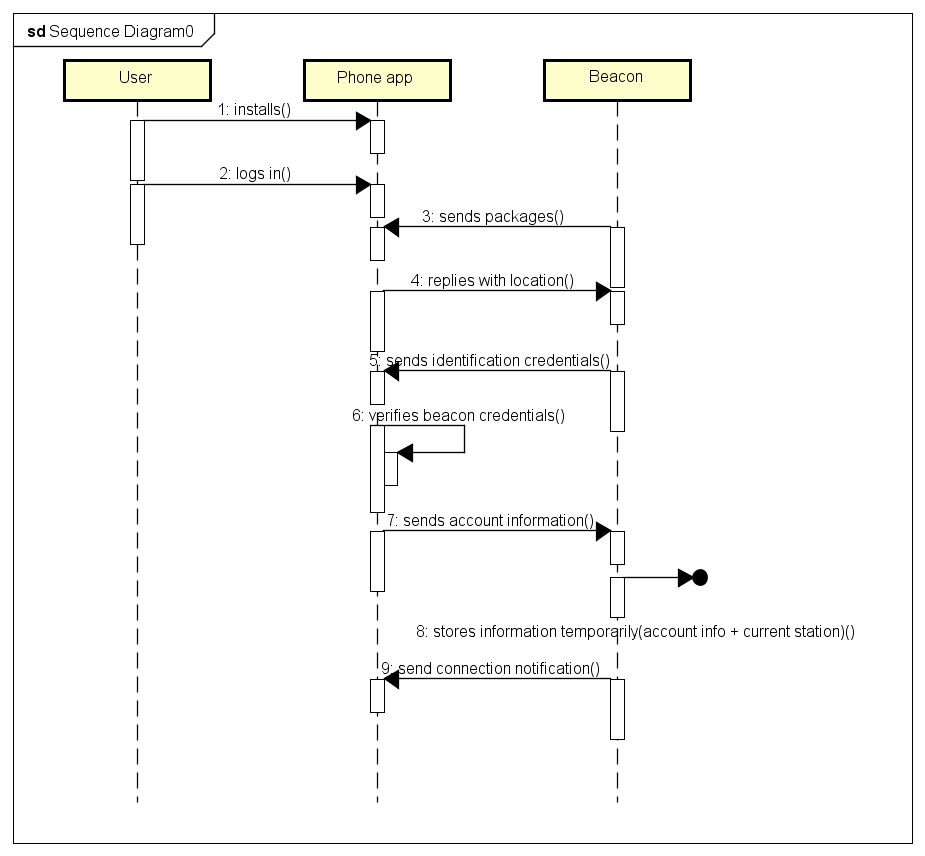
\includegraphics[width=\textwidth]{Pictures/seq_diagram_uc1.png}
	\caption{System sequence diagram- use case 1(Connect phone to beacon)}
	\label{fig:seqDiagram1}
\end{figure}
Figure \ref{fig:seqDiagram1} is a direct mapping of use case 1(connect phone to beacon).

\begin{figure}[H]
	\centering
	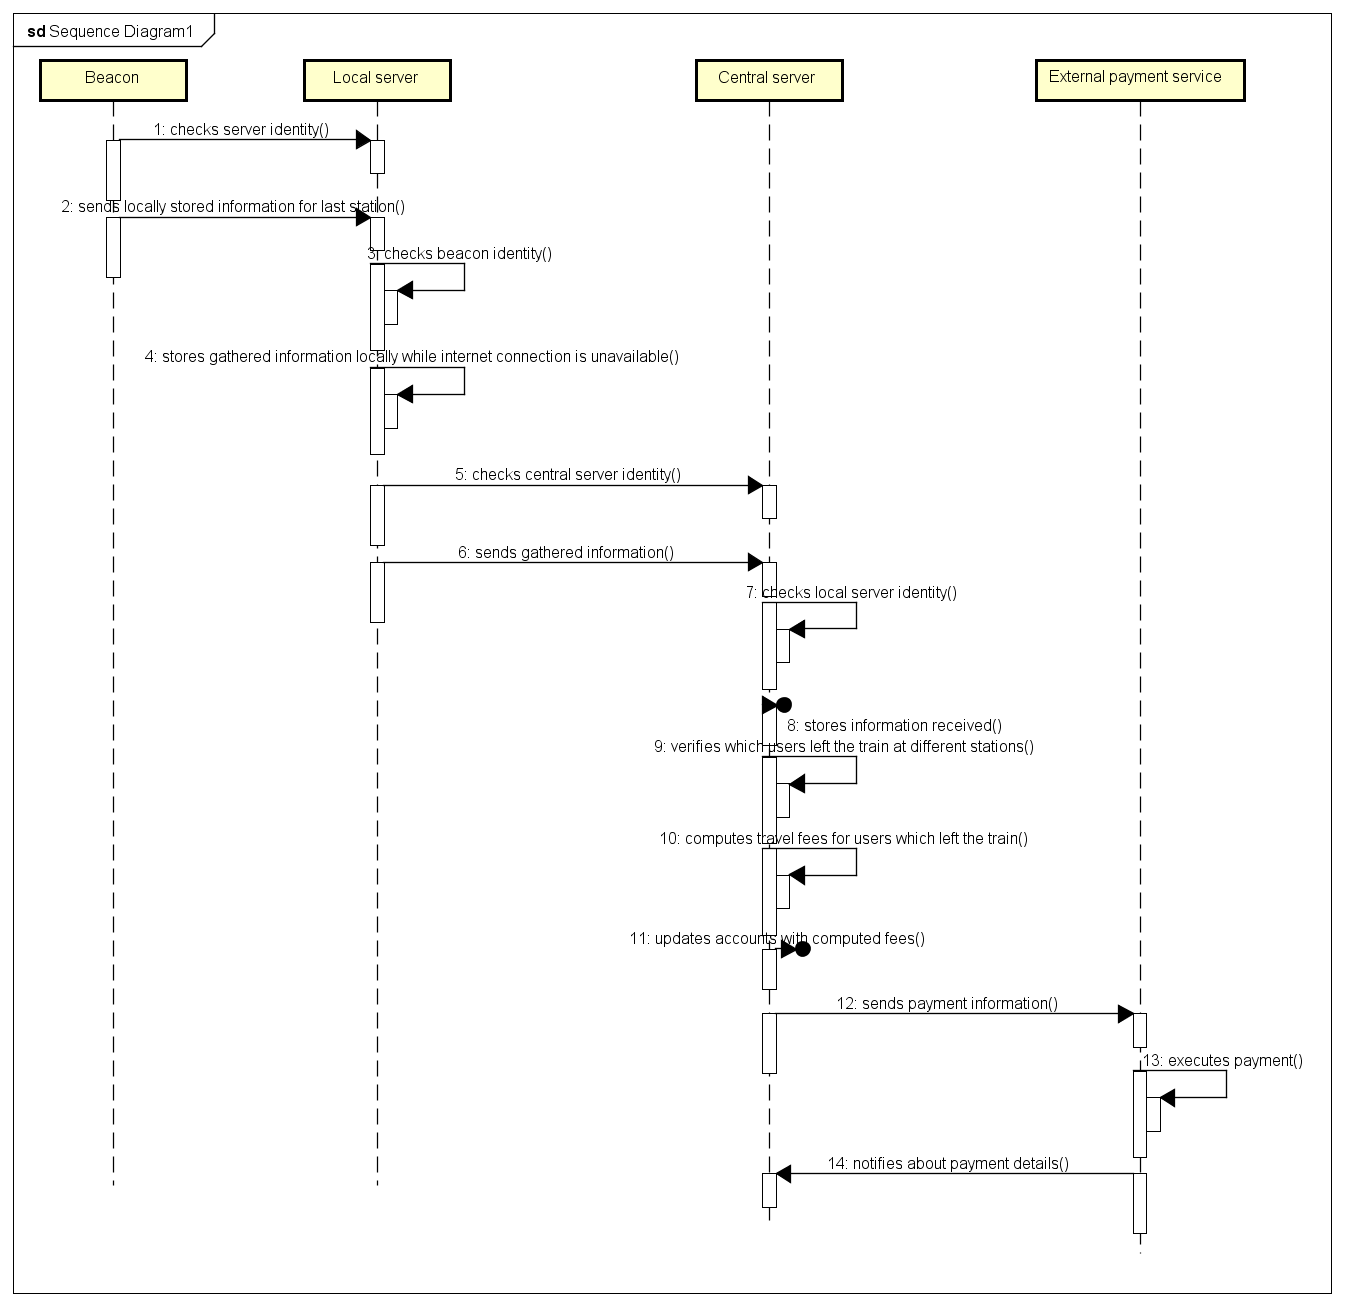
\includegraphics[width=\textwidth]{Pictures/seq_diagram_payment.png}
	\caption{System sequence diagram- payment}
	\label{fig:seqDiagram2}
\end{figure}
Figure \ref{fig:seqDiagram2} displays the information flow corresponding to use cases "Disconnect from beacon" "Calculate travel fee" and "Make payment". For this process, the system uses a third party payment service.

\begin{figure}[H]
	\centering
	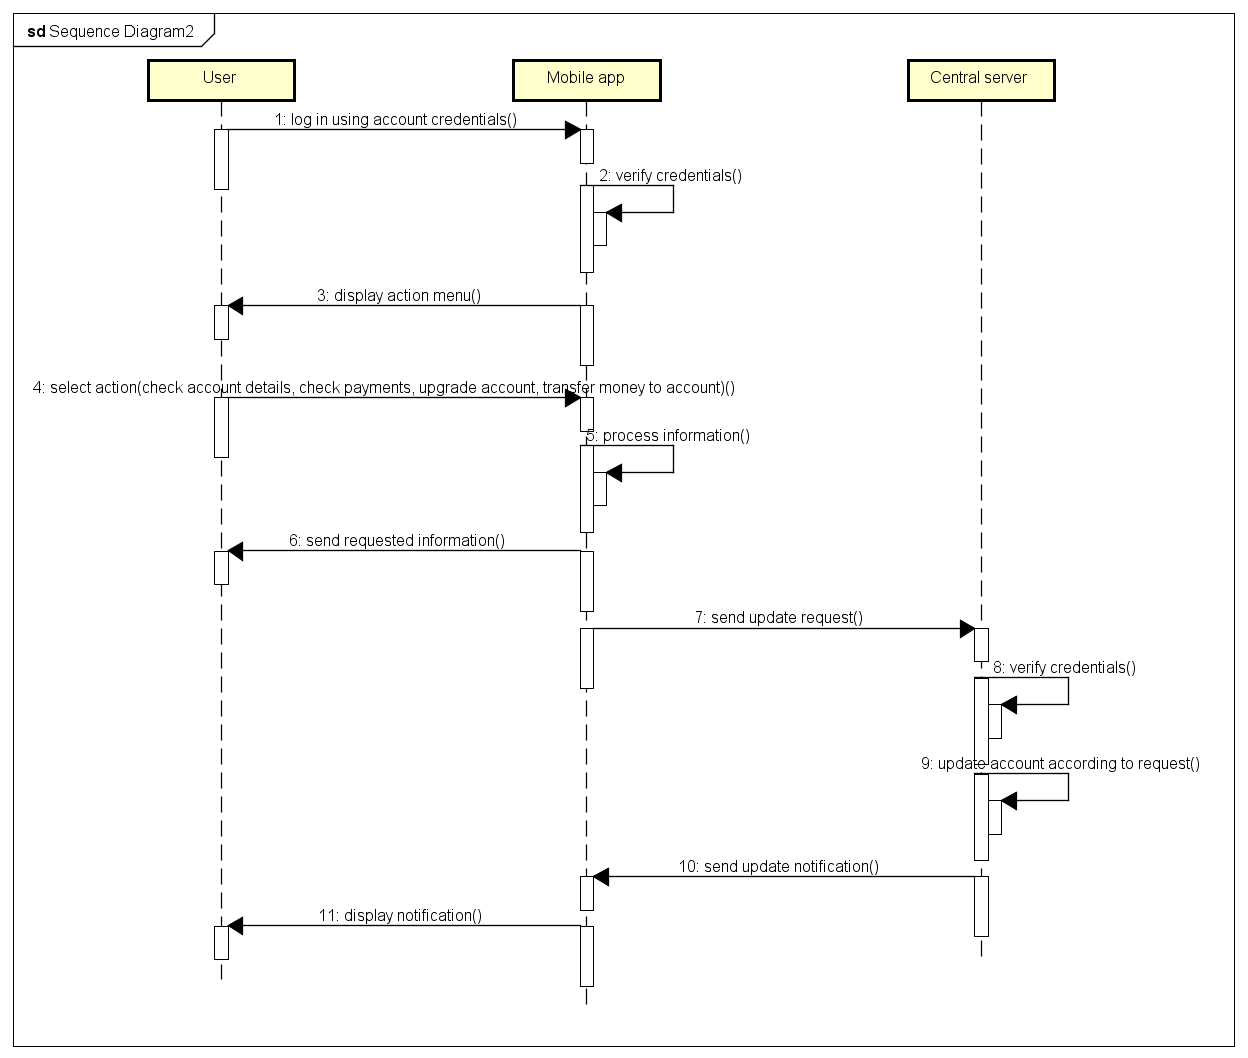
\includegraphics[width=\textwidth]{Pictures/seq_diagram_checkAccount.png}
	\caption{System sequence diagram- Check account details}
	\label{fig:seqDiagram3}
\end{figure}
Figure \ref{fig:seqDiagram3} displays the information flow related to use cases "Register through application", "Check account balance" and "Login through application". This process describes the general outline for different actions the user can perform using the mobile application.


\begin{figure}[H]
	\centering
	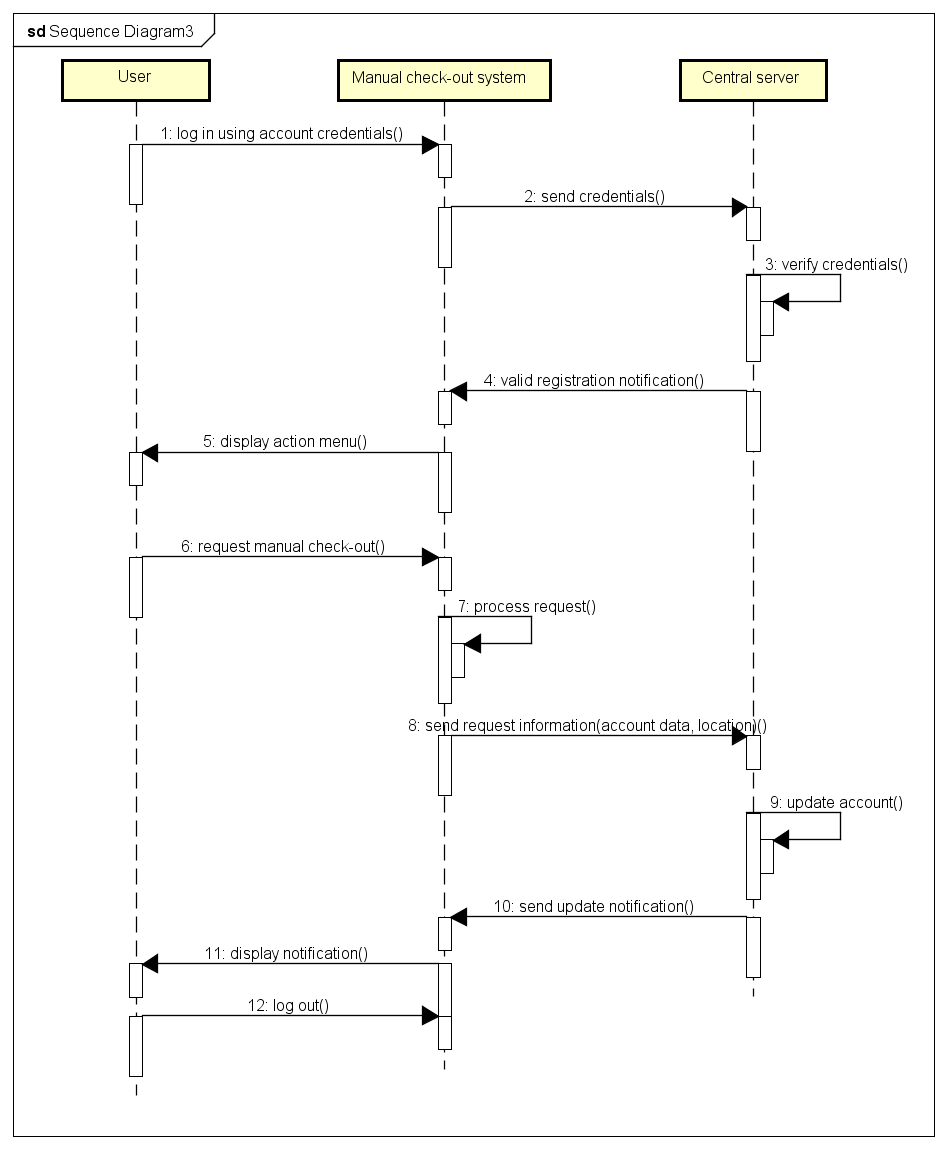
\includegraphics[width=\textwidth]{Pictures/seq_diagram_manualCheckOut.png}
	\caption{System sequence diagram- Manual checkout}
	\label{fig:seqDiagram4}
\end{figure}
Figure \ref{fig:seqDiagram4} shows the main information flow corresponding to the use case "Manually sign out from journey". This use case was designed as an alternative to the main "Disconnect from beacon" use case which will give users the possibility to manually check out at a particular train station in case of the phone to beacon connection not being available.

%\section{Data View}-- what is data view?
%\section{Physical View}